%导言区
\documentclass{article}%book,report,letter
\usepackage{ctex}

\usepackage{amsmath}
%\ctexset{section = {format={\Large\bfseries}}}
\usepackage{multicol}%用于实现在同一页中实现不同的分栏 
\usepackage{authblk}
\usepackage{cite}%参考文献引用
\usepackage{graphicx}%插入图片
\usepackage{caption}
% 设置页面的环境,a4纸张大小,左右上下边距信息
\usepackage[a4paper,left=10mm,right=10mm,top=20mm,bottom=20mm]{geometry}


\makeatletter
\def\@captype{figure}
\makeatother

\newenvironment{figurehere}
	{\def\@captype{figure}}
	{}
\makeatother%用于连接公式编号

\title{\heiti 双车协同智能控制系统}
\author{\kaishu 王子豪 \hspace{1em} 李铮 \hspace{1em} 颜斌}
\affil{(杭州电子科技大学\quad 电子信息学院, 浙江杭州, 310018)}
\date{}%不要日期


%正文区(文稿区)
\begin{document}
	\maketitle	
	%摘要
	\noindent\textbf{摘要:}
	本系统以单片机CH32V307VCT6为核心控制器,双车使用数字摄像头(MT9V034)采集道路信息,位于基础道路时双车均采用提取边缘法检测赛道并通过图像处理正常行驶,特殊路段时双车可采用电感检测区域的电磁线实现道路检测。并且双车可通过TOF测距模块检测坡道和路障,适应不同道路状况。双车均通过编码器监测自身车辆的实时速度,使用 PID 控制算法调节电机的转速和舵机的打角,实现智能车在运动过程中速度和方向的控制。同时,为应对突发事件,本系统提供前车无线供电后车的方案。在运行过程中两辆车之间通过 CH9141蓝牙通信模块传输数据和超声波模块检测车辆之间的距离以实现双车协同运行。本系统旨在实现两辆小车在自动识别道路的条件下,有序而安全的高速行驶。
	\newline%另起一行
	%关键字
	\textbf{关键字:}双车协同; PID算法; 图像处理; 智能车
	
	\setcounter{section}{-1}%使标题从0开始
		
	\begin{multicols}{2}%开启分两栏格式
		
		
		\section{引言}%*标题无序号	
		智能汽车自动驾驶技术是汽车行业发展的跨时代标志,推动汽车行业走向智能化方向发展的道路\textsuperscript{\cite{ref1}}。随着科技的发展,人们对智能汽车的需求也趋于多元化,不再局限于解决道路拥堵和节能环保等方面,智能车逐渐成为代替人们在危险环境进行探索和开发有限资源的重要工具。但单智能车存在不能高效执行并行度高且复杂的任务的缺点,所以多车协同系统得到学者们的广泛关注\textsuperscript{\cite{ref2}}。为了深入研究多车协同合作时遇到的难题,本文在CH32V307单片机主控下自主设计并实现了双车协同智能控制系统,通过多模块检测距离和蓝牙通信,保持队列秩序,同时设计摄像头图像处理算法和电磁感应处理算法,完善双重道路判断,同时通过无线充电解决极端条件问题,真正实现高稳定性和高速度的双车协同系统。
		
		\section{系统总体方案设计}
		本系统总体方案设计如图1所示,整体分为三个板块:道路信息采集与处理;车辆控制与运行;双车协同与交互信息。该系统核心控制器为沁恒CH32V307VCT6单片机,通过数字摄像头和电磁传感器采集道路信息,配合激光传感器进行道路元素识别,并控制前轮舵机模块和后轮电机模块实现智能车的正常行驶。双车协同方案以蓝牙交互信息和超声波模块测距为核心。系统整体分为六大模块。	
		
		主控模块,作为整个智能汽车的“大脑”,将采集摄像头、TOF和电磁传感器的信号,根据控制算法做出控制决策,驱动直流电机和舵机完成对智能汽车的控制。
			 
		传感器模块,是智能汽车的“眼睛”,可以通过一定的前瞻性,提前感知前方的赛道信息,为智能汽车的“大脑”做出决策提供必要的依据和充足的反应时间。 		
			
		电源模块,为整个系统提供合适而又稳定可靠的电源。
							
		电机控制模块,驱动电机完成智能汽车的加减速控制和转向控制。 
				
		双车协同模块,实时获取双车距离,蓝牙通信交互配合,同时实现双车无线充电功能。 	
				
		辅助调试模块,主要用于智能汽车系统的功能调试,参数设置,状态监控。
		
		该系统通过MCU将多个模块协同工作,实现高稳定性和高速度的双车协同运作。
		
		\begin{center}
			\centering{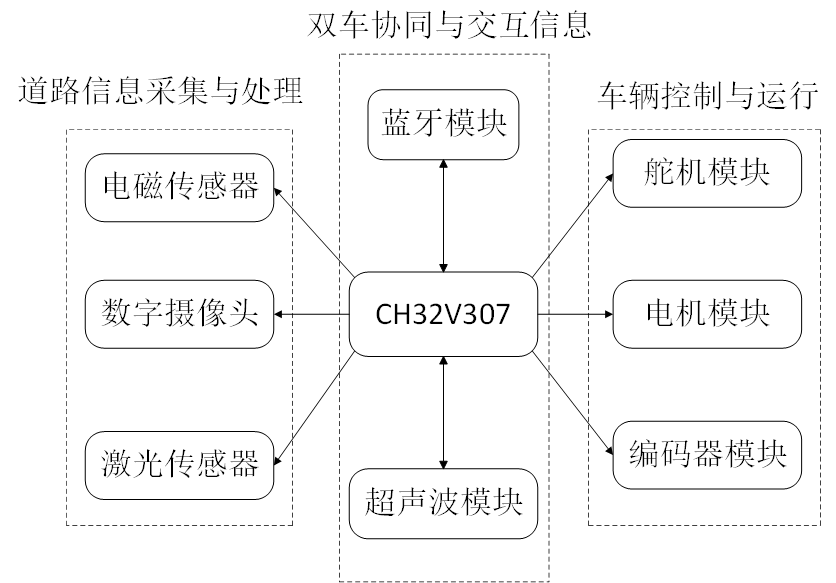
\includegraphics[scale=0.4]{image/my_system.png}}
			\caption{系统总体方案框图}
		\end{center}
		
		\begin{center}
			\centering{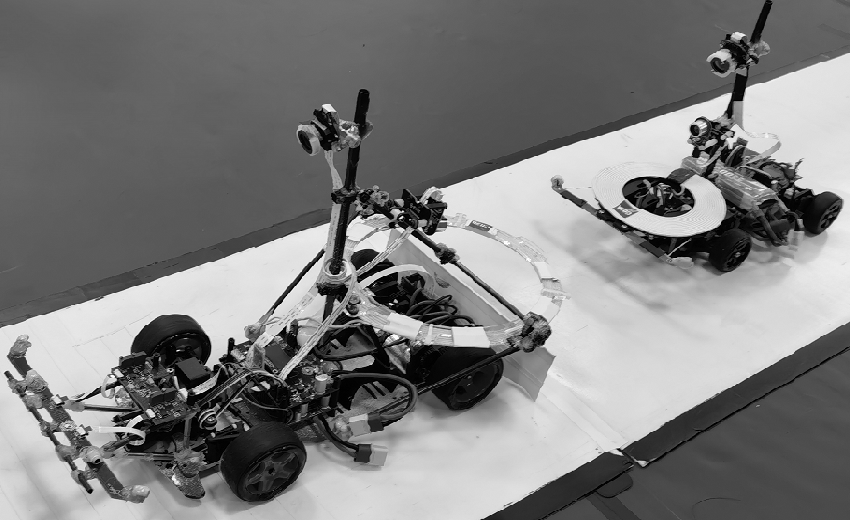
\includegraphics[scale=0.4]{image/twocar_system.png}}
			\caption{实际车模图}		
		\end{center}
		
		
		\section{系统硬件电路设计}
		
		\subsection{硬件电路总体设计}
		硬件总体设计采用CH32V307为核心运算的设计方案,整套硬件系统可共分为3大模块,分别为电源模块、传感器模块、驱动模块。
		本文借助 WCH 芯片技术手册,对硬件电路设计完善的系统。图3是主控芯片原理图:
		\begin{center}
			\centering{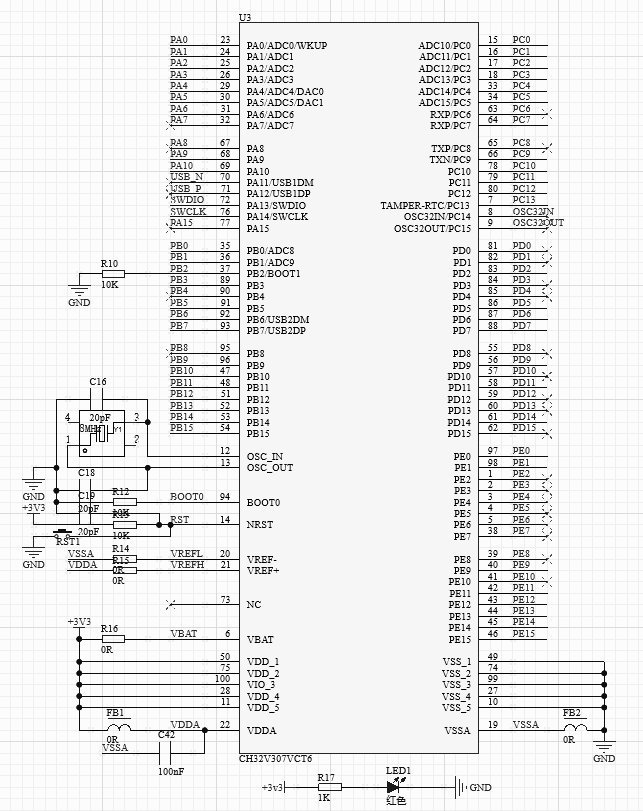
\includegraphics[scale=0.40]{image/mcu.jpg}}
			\caption{主控芯片原理图}		
		\end{center}		
		\subsection{系统电源设计}
		根据系统设计, 5V电源选择TPS7A8001,高性能超低压差线性稳压器TPS7A8001工作在-0.3V至6.5V的输入电压范围内,提供超低压差,高输出电流和低地电流。
		
		3.3V电源使用TPS7333,具备超低静态电流和睡眠状态电流,输出电流最大可达500mA。
		
		舵机电源本系统采用TPS5450作为开关电源,优点在于转换效率高,能量损耗小,最大能输出5A电流。TPS5450不仅为舵机提供稳压电源,同时也作为唯一的前级电源,作为5V电源和3.3V电源的输入。
		
		具体电源模块设计如图4所示。
		\begin{center}
			\centering{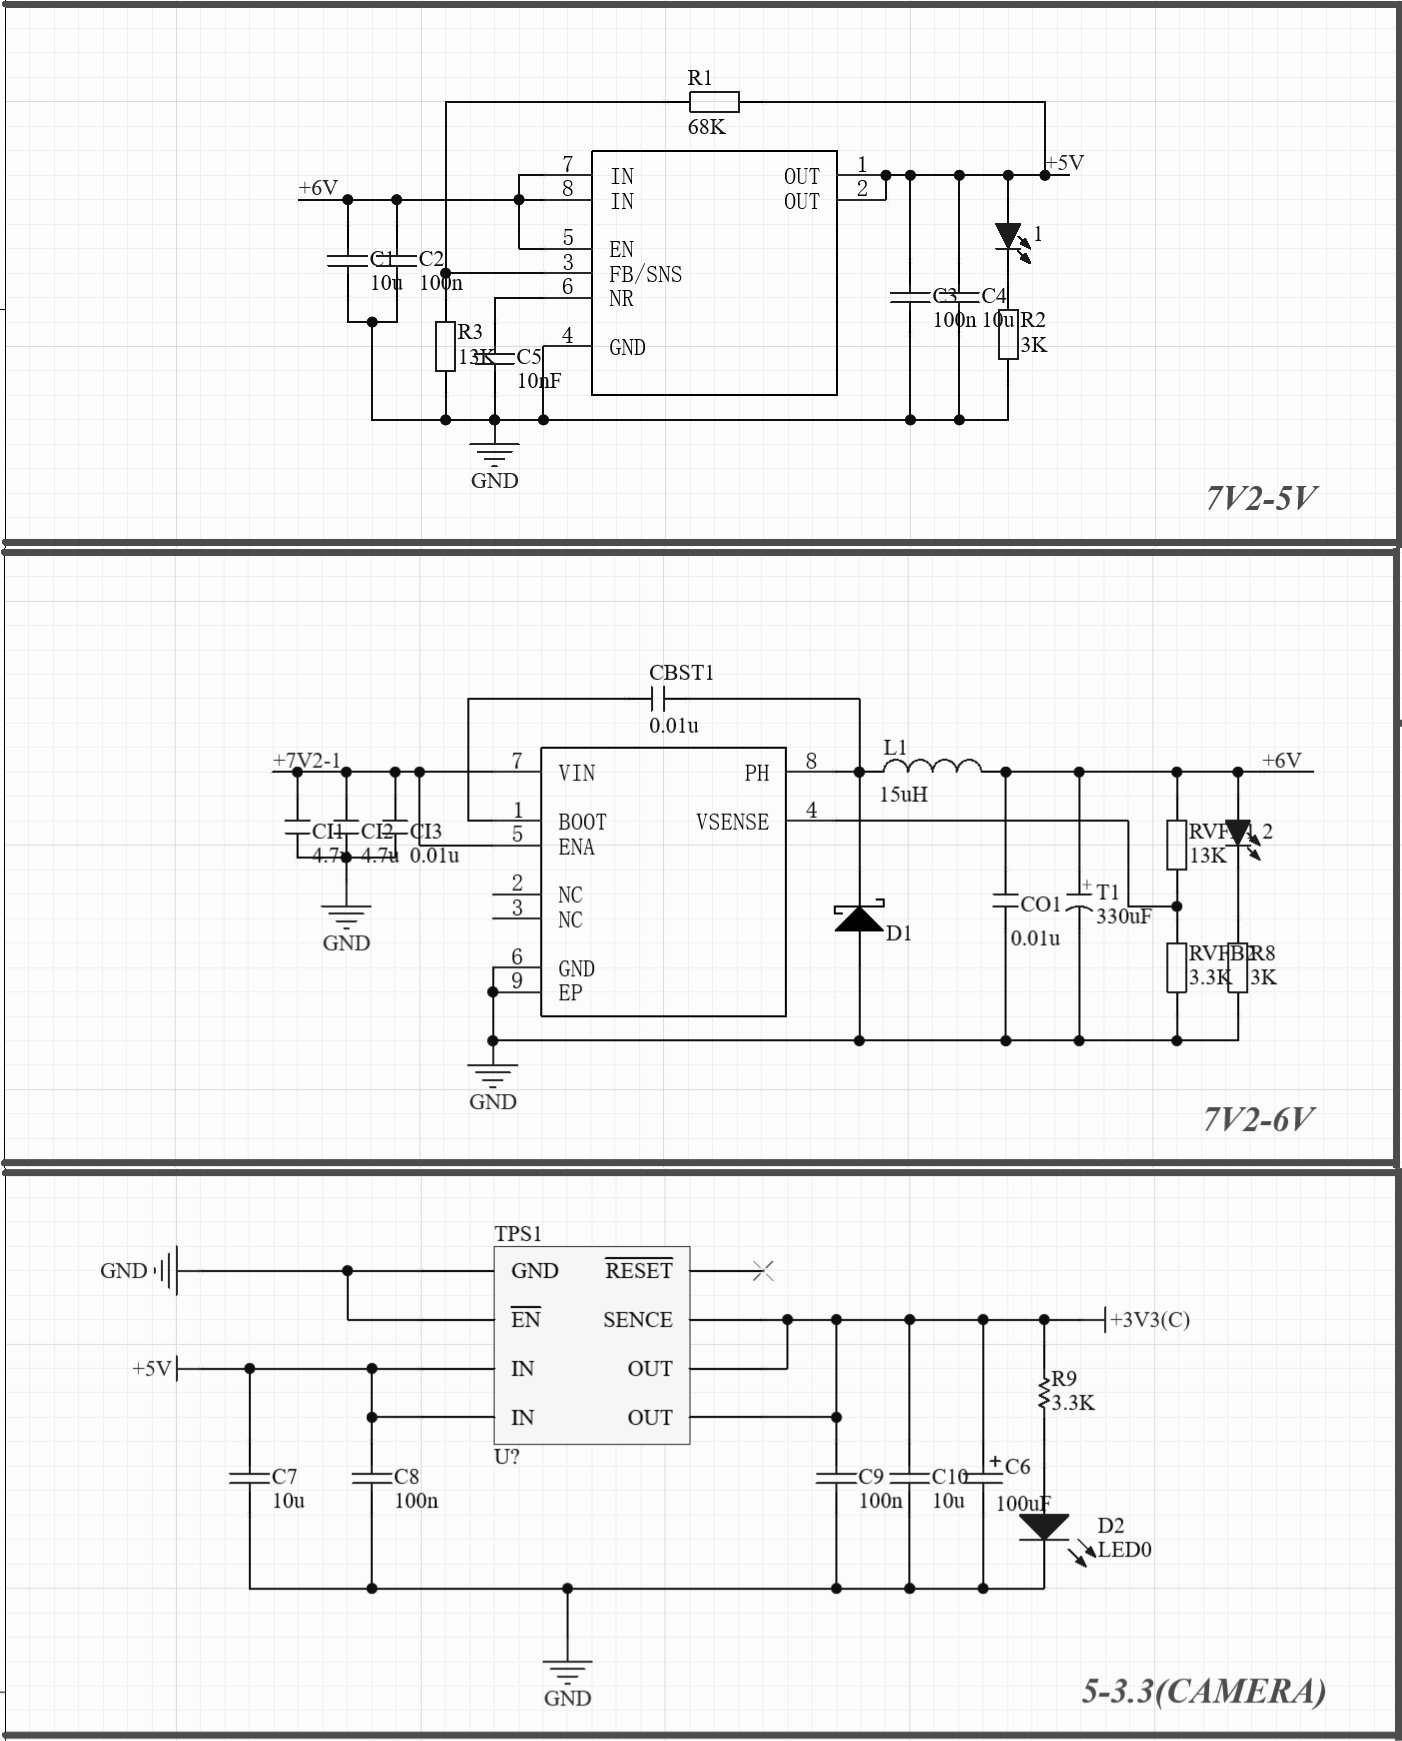
\includegraphics[scale=0.20]{image/power_source.jpg}}
			\caption{电源模块设计图}		
		\end{center}
		
		
		\subsection{传感器接口设计}
		本系统硬件提供多模块接口,包括:驱动板接口、舵机接口、电磁运放板接口、摄像头接口、OLED屏接口、TOF接口、超声波接口、发射端使能接口、蓝牙接口和SD卡接口,具体传感器模块接口设计如图5所示。
		\begin{center}
			\centering{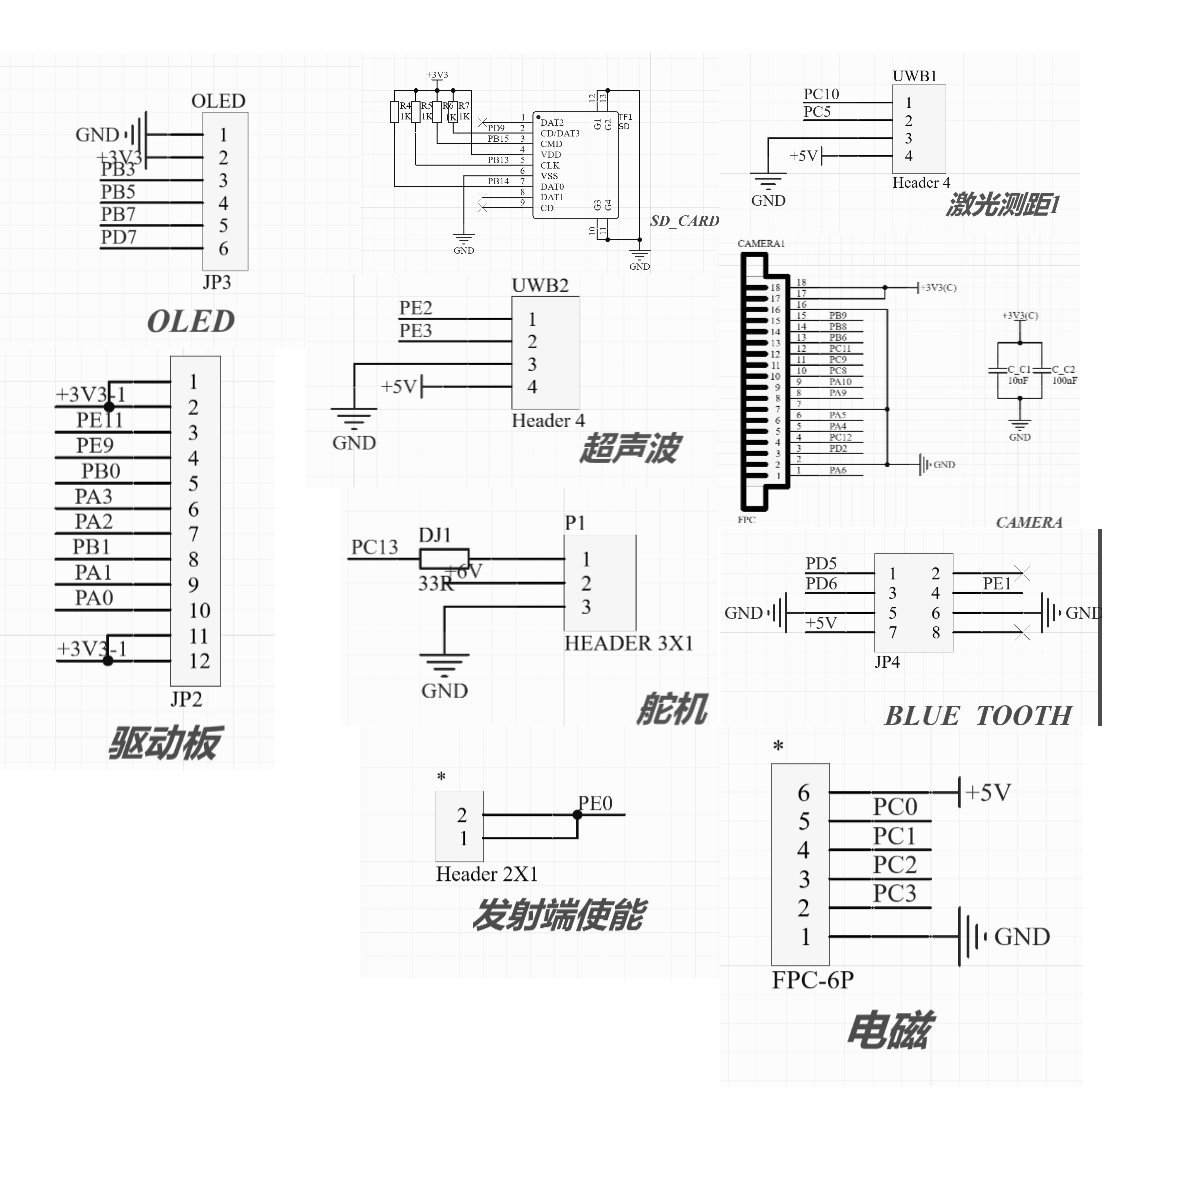
\includegraphics[scale=0.20]{image/multi_interface.jpg}}
			\caption{主要模块接口设计图}		
		\end{center}
		
		\subsection{驱动电路设计}
		
		\subsubsection{电磁运放电路}
		
		电磁线的信号由LC并联谐振得到,为模拟信号,由于电感感应出来的感应电动势比较小而且是差分信号,所以需要放大电路进行调理。
		
		本系统最终采用双电源仪表放大器\textsuperscript{\cite{ref3}}方案,直接放大差分信号,优点是共模抑制比高,线性度高,失调电压小。从仪表放大器出来的信号是类似正弦波的信号,为了将该信号转化成直观的直流电平,系统选择运放检波方案。具体电磁运放电路图如图6所示:
		
		\begin{center}
			\centering{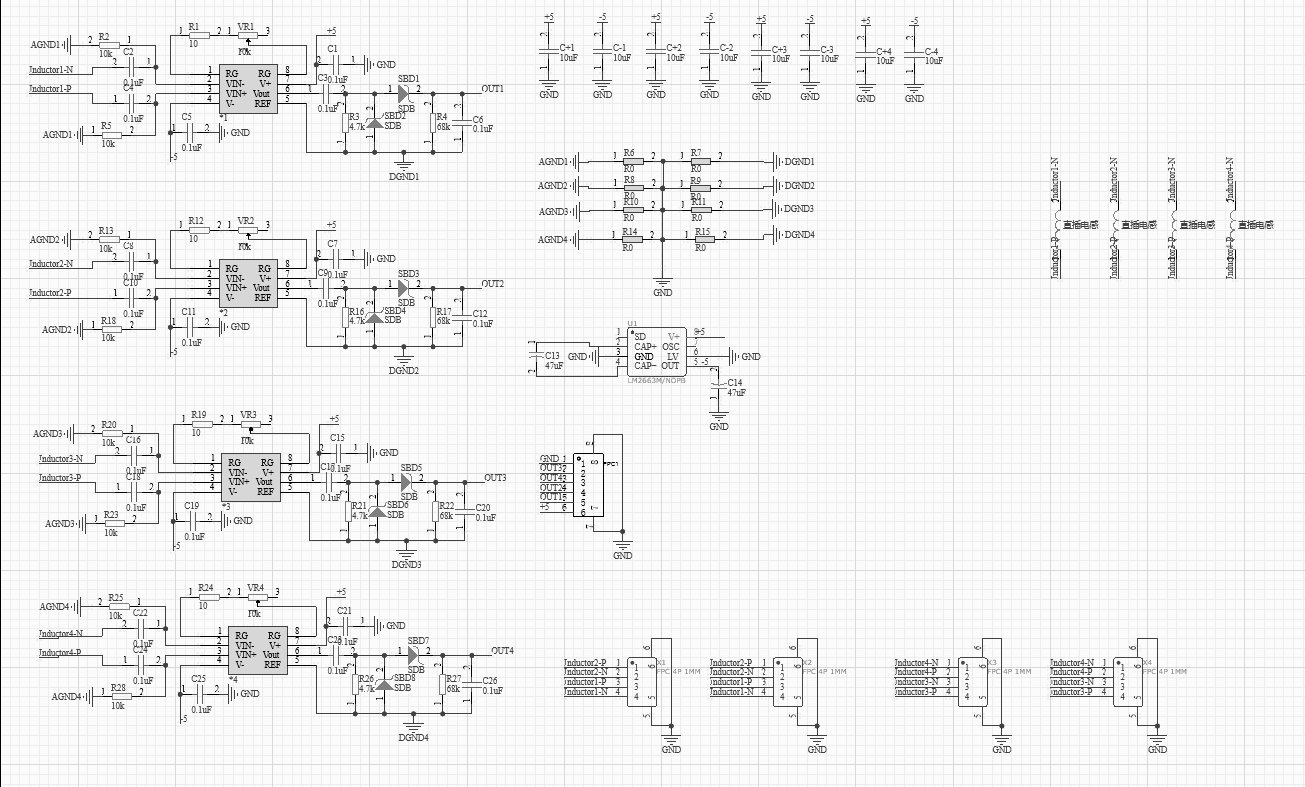
\includegraphics[scale=0.2]{image/电磁运放电路.jpg}}
			\caption{电磁运放电路图}		
		\end{center}
		
		\subsubsection{无线充电发射端与接收端电路}
		
		无线充电方案发射端如图7所示:
		\begin{center}
			\centering{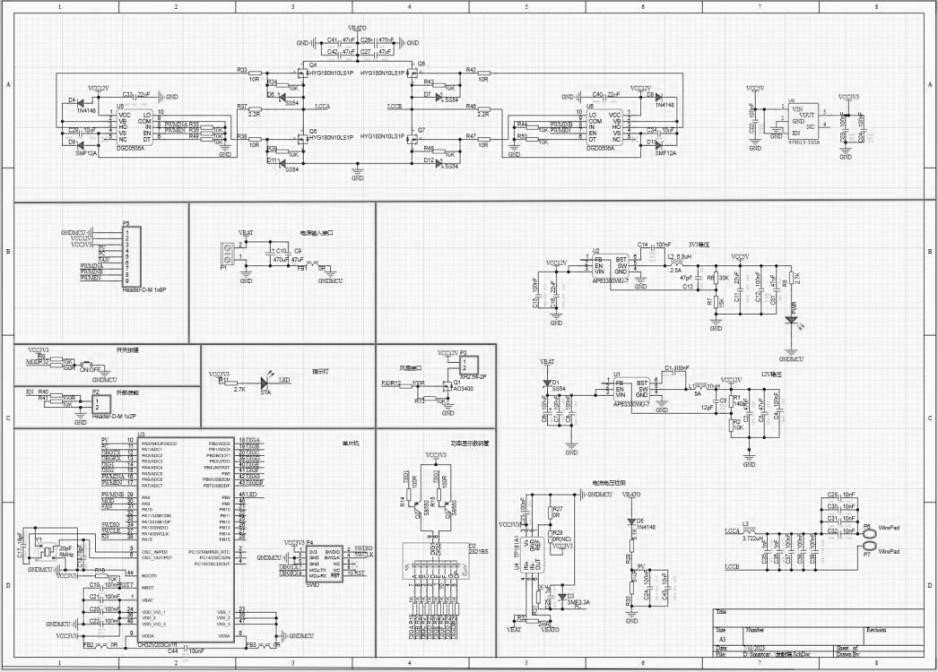
\includegraphics[scale=0.3]{image/发射端电路.jpg}}
			\caption{充电发射端电路图}		
		\end{center}
		
		无线充电方案接受端如图8所示:
		\begin{center}
			\centering{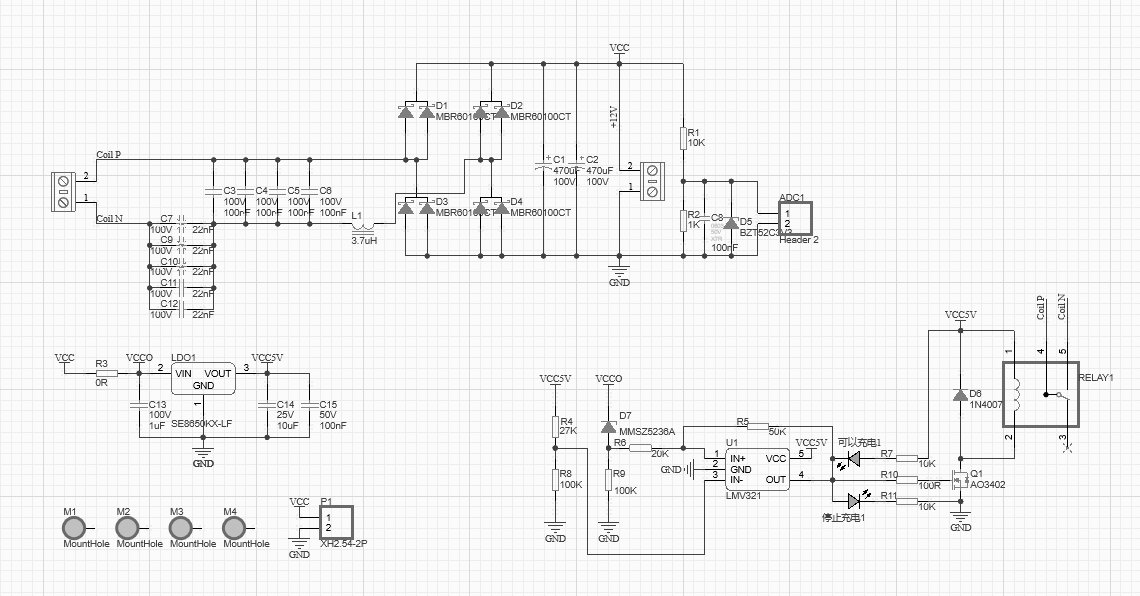
\includegraphics[scale=0.25]{image/接收端电路.jpg}}
			\caption{充电接收端电路图}		
		\end{center}
		
		\subsubsection{驱动板电路}
		
		对于电机驱动电路,有多种选择,例如专用电机驱动芯片MC33886、L298N等,但是以上芯片集成度高,导通内阻大,瞬间电流小,驱动效果差。因此本系统选择用H桥\textsuperscript{\cite{ref4}}的全桥电路,使智能车拥有及时刹住的能力,减速入弯。此外,本系统选用电机型号为RN-380,通过大量测试,数据表明汽车启动和堵转时电流可以达到5A(适当的驱动频率下)。开始系统采用英飞凌的集成半桥芯片 BTS7960B构成H桥来驱动电机,由于速度提升后电机耗电较大,发热严重,同时BTS的成本相对较高。最终系统选择4N-MOS搭的H桥方案,采用内阻小的4片NMOS来搭建的2个H桥使得单电机驱动问题彻底解决。具体电磁运放电路图如图9所示:

		\begin{center}
			\centering{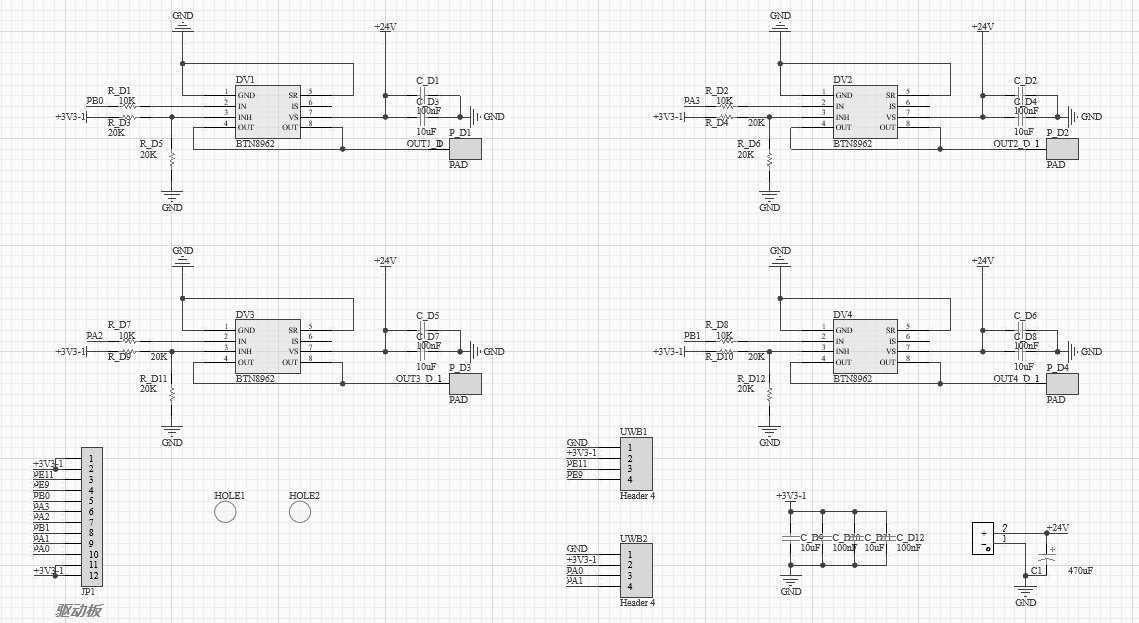
\includegraphics[scale=0.20]{image/驱动板电路.jpg}}
			\caption{驱动板电路图}		
		\end{center}
				
		\section{系统软件设计}
		系统软件设计部分由无线充电、道路信息采集与处理、舵机转向控制、电机速度控制和双车协同交互五大模块组成。系统程序流程图如图10所示,系统对各模块初始化后开始对后车进行无线充电;接收到充电完成的信号后进行正常的道路信息采集与处理,结合舵机转向控制和电机驱动控制,智能车队稳定、有序而安全的行驶在道路中央;在识别到车库元素后,前车停在车库附近,后车停入车库,系统结束运行。	
			\begin{center}
				\centering{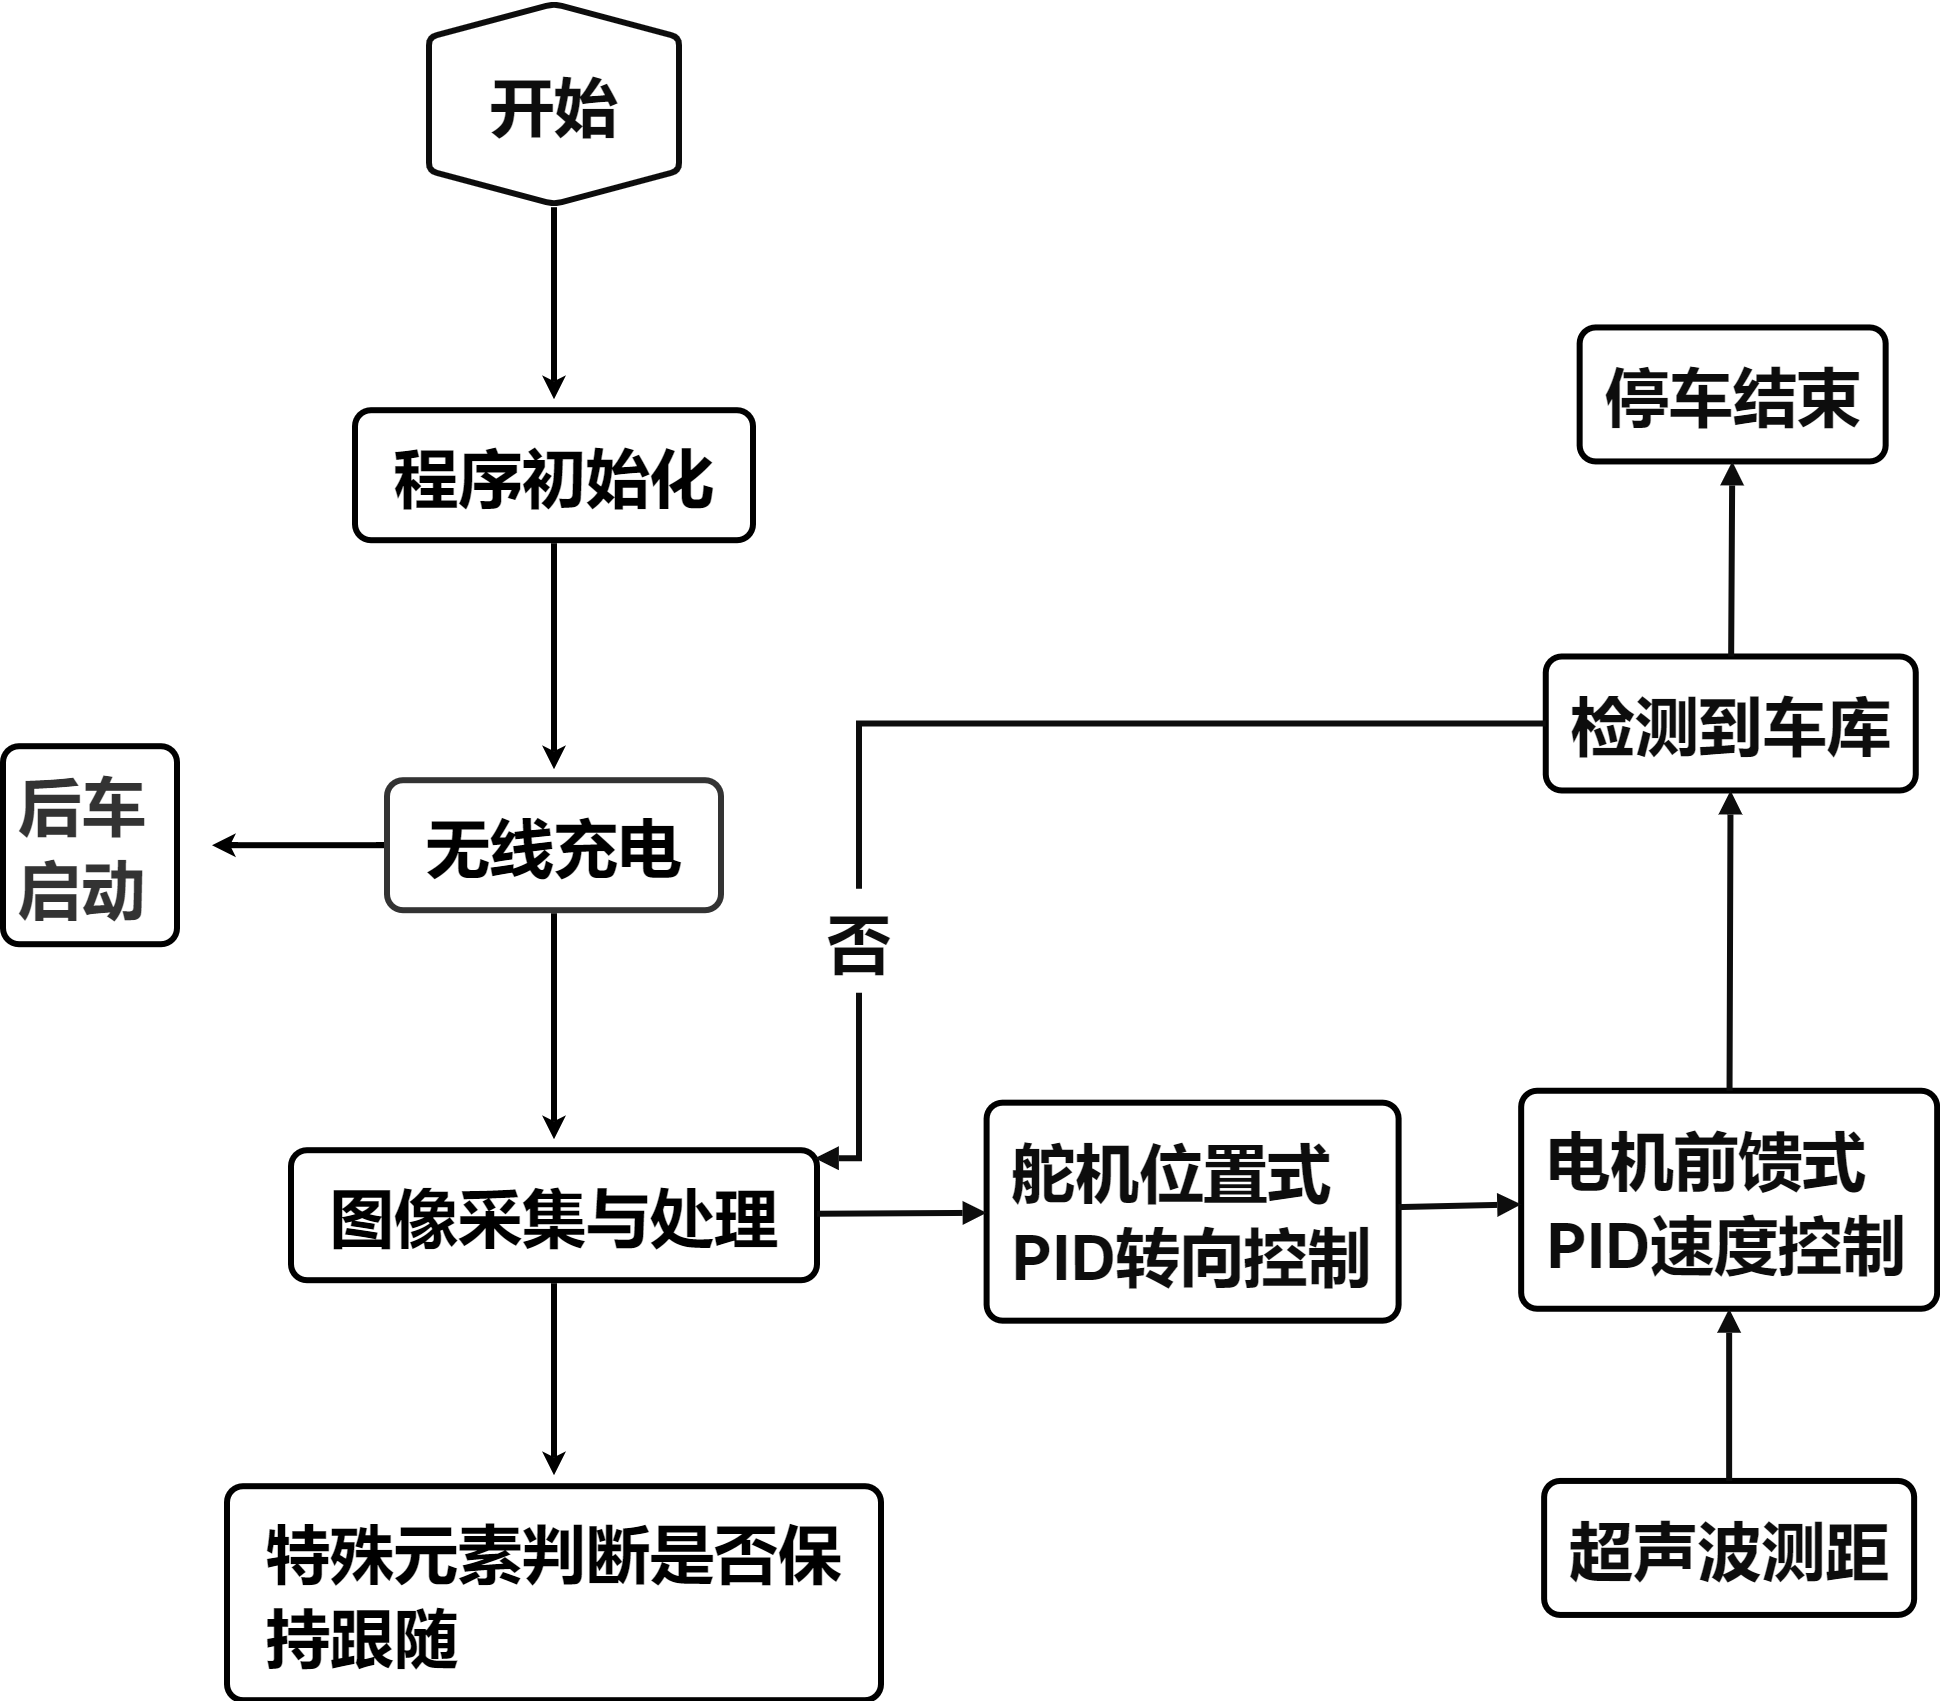
\includegraphics[scale=0.35]{image/开始.png}}
				\caption{系统程序流程图}		
			\end{center}				
		\subsection{道路信息采集与处理}
		
		\subsubsection{图像采集}
		本系统选择MT9V034数字摄像头作为图像传感器,这款宽VGA CMOS图像传感器采用ON SEMICONDUCTOR突破性的低噪点CMOS成像技术,实现了CCD图像质量(基于信噪比和低感光度)的同 时,还保持了CMOS的固有尺寸、成本和集成优势,成为道路图像采集传感器的理想选择。可通过主控芯片使用两线总线协议对寄存器进行配置,可设置图像采集时的曝光时间、增益灵敏度等工作参数,并可开启全局快门和高动态范围操作。在默认模式下的图像输出速度为每秒50帧\textsuperscript{\cite{ref5}}。
		
		\subsubsection{图像处理}
		由于数字MT9V034摄像头直接采集的原始图像为灰度图,本系统先通过多局部去噪处理降低图像噪声的干扰,增强图像信息的一致性,再采用大津法确定图像二值化分割阈值过滤非必要图像信息。大津法( OTSU)最早是由日本学者大津在1979年提出的,基本的思想是在图像灰度差异的基础上,自动选取合适的阈值,将图像分为背景和目标两个部分\textsuperscript{\cite{ref6}}。使用大津法得到的道路二值化图像如图11所示。
		\begin{center}
			\centering{
\includegraphics[scale=2.00]{image/basic_road.png}}
			\caption{道路二值化图像}		
		\end{center}
		
		赛道边沿的提取是所有识别以及控制的基础,根据摄像头所采集的图像是近大远小这个特点,我们对赛道边沿提取时先从近几行入手,根据近处的边线给定远处边线的寻找范围,通过阈值判断找出下一行的准确边界,从而提取赛道的中线。最终边缘提取得到的道路轮廓图如图12所示。
		\begin{center}
			\centering{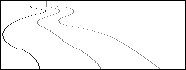
\includegraphics[scale=1.20]{image/basic_edge.jpg}}
			\caption{道路轮廓图像}		
		\end{center}
		
		通过特殊的图像算法,我们能够精准的识别不同的道路元素,同时优化运行路径和稳定性,常见元素存在:十字、环岛、车库、断路,配合专门的tof激光测距模块我们也能识别较为特殊的道路元素:坡道和路障。	
		\newline%另起一行4
		十字元素原始图像和处理后的图像如图13所示:	
		\begin{center}
			\centering{
\includegraphics[scale=0.30]{image/crossroad.jpg}}
			\caption{十字元素}		
		\end{center}	
		环岛元素原始图像和处理后的图像如图14所示:
		\begin{center}
			\centering{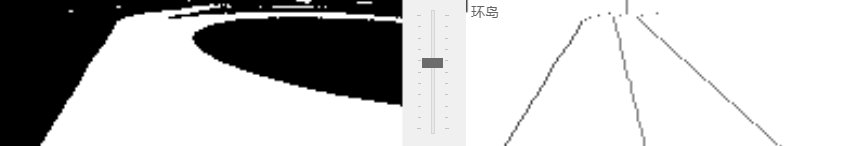
\includegraphics[scale=0.30]{image/round_road.jpg}}
			\caption{环岛元素}		
		\end{center}	
		车库元素原始图像和处理后的图像如图15所示:
		\begin{center}
			\centering{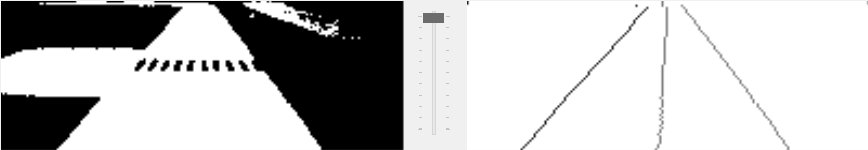
\includegraphics[scale=0.30]{image/garage.jpg}}
			\caption{车库元素}		
		\end{center}	
		断路元素原始图像和处理后的图像如图16所示:
		\begin{center}
			\centering{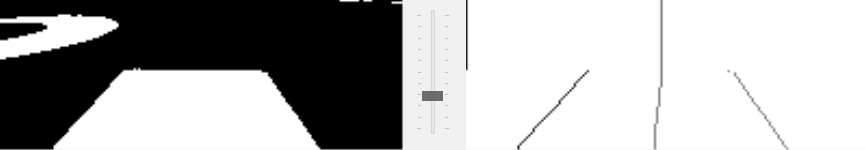
\includegraphics[scale=0.30]{image/breakroad.jpg}}
			\caption{断路元素}		
		\end{center}
		坡道元素原始图像和处理后的图像如图17所示:
		\begin{center}
			\centering{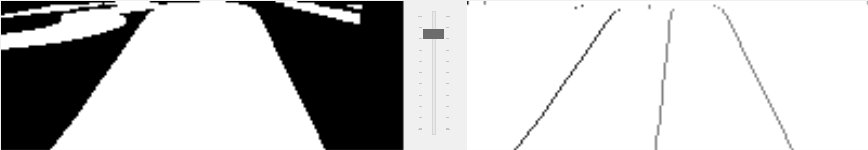
\includegraphics[scale=0.30]{image/ramp.jpg}}
			\caption{坡道元素}		
		\end{center}
		路障元素原始图像和处理后的图像如图18所示:
		\begin{center}
			\centering{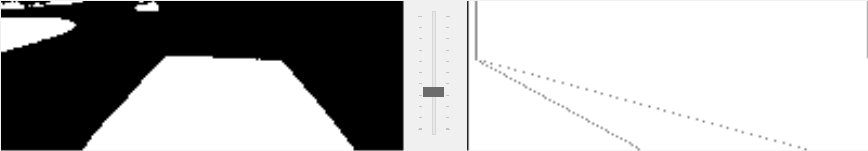
\includegraphics[scale=0.30]{image/roadblock.jpg}}
			\caption{路障元素}		
		\end{center}
		
		\subsection{舵机转向控制}
		
		舵机是一个位置随动系统,由舵盘、减速齿轮组、位置反馈电位计、直流电机和控制电路组成。通过内部位置反馈,使舵盘输出转角正比于输入的控制信号。在负载小于其最大输出力矩的情况下,舵机的输出转角正比于输入信号的脉冲宽度。舵机控制是控制算法中最重要的方面之一,本系统舵机的控制采取传统的 PID 控制。基于偏差的比例(Proportlonal)、积分(Integral)和微分(Derivative)的 控制器简称为PID控制器。其是工业过程控制中最常见的一种过程控制器。由于PID 控制器算法简一单、鲁一棒性强,因而被广泛应用于化工、冶金、机械、热工和轻工等工业过程控制系统中\textsuperscript{\cite{ref7}}。常规PID控制系统原理图如19所示。
		
		\begin{center}
			\centering{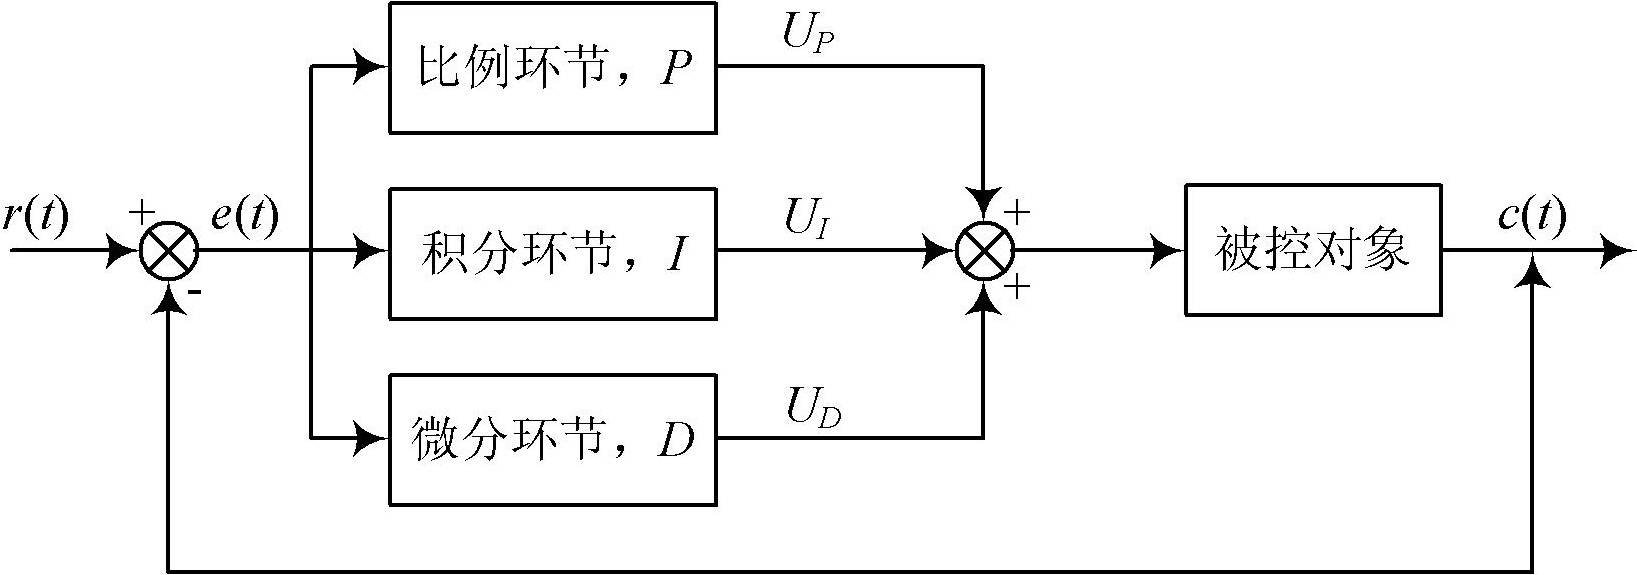
\includegraphics[scale=0.235]{image/PID.jpg}}
			\caption{常规PID控制系统原理图}		
		\end{center}

		随着微型计算机的出现,特别是现代嵌入式微处理器的大量应用,实现了由模拟PID控制器到数字PID控制器的转变。数字PID控制器在实际应用中可分为两种:位置式PID控制器和增量式PID控制器\textsuperscript{\cite{ref7}}。本系统对舵机的控制采用位置式PID,具体算法实现公式如式(1)。
		 P I D  公式展示:
		\begin{equation}
			u(t)=K_{p} e(t)+\frac{K_{p}}{T_{t}} \int_{0}^{t} e(t) d t+K_{p} T_{D} \frac{d e(t)}{d t}
		\end{equation}		
		
		其中  $K_{p}$  为比例时间系数
		
		其中  $K_{i}=\frac{K_{p}}{T_{t}}$ 为积分时间系数
		
		其中  $ K_{d}=K_{p} T_{D} $ 为微分时间系数
		
			
		\subsection{电机速度控制}
		\subsubsection{差速系统}
		大量的研究和实验表明,较为简单的PID控制差速在汽车高速状态下逐渐展现疲态,纯粹的调整PID的参数已经无法提升汽车速度的上限。而本系统采用的阿克曼转向系统是目前四轮汽车较为普遍的差速转向系统,拥有更强的稳定性和更高的速度上限。阿克曼原理是在不考虑汽车质心侧偏、汽车行驶过程 中的侧向力、横摆角和极端恶劣的路况下,车辆无论是直行 还是在拐弯时,如果每个车轮的运动轨迹都可以完全符合 它的自然运动轨迹,那么就可以保证轮胎与地面间处于纯滚动而无滑移现象\textsuperscript{\cite{ref8}}。阿克曼转向结构原理图如图20所示:
		
		\begin{center}
			\centering{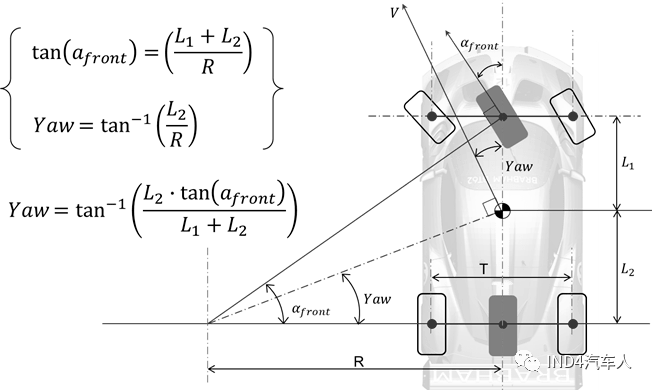
\includegraphics[scale=0.40]{image/Akman.png}}
			\caption{阿克曼转向系统图}		
		\end{center}
		
		\subsubsection{电机控制}
		本系统采用闭环电机控制,通过配合编码器,实现速度精确控制。具体算法中,电机速度控制采用了增量式PID 加 pwm 前馈控制的方法。增量式 PID 控制算法的表达式如以下公式所示:
		\begin{equation}
			\Delta(k) = u(k)-u(k-1)
		\end{equation}	
		则:
		\begin{equation}					
			\begin{split}				
				&\Delta u(k) = K P e(k)+K P T T I \sum e(i) k i = 0+K P T D T \\
				&[e(k)-e(k-1)]-K P e(k-1)-K P T T I \Sigma e(i) k-1 i = 0 \\
				& -K P T D T[e(k-1)-e(k-2)] 
			\end{split}
		\end{equation}						
		令:
		\begin{equation}
			 K I = K P T T I ; K D = K P T D T 
		\end{equation}
		则:	
		\begin{equation}
			\begin{split}	
				&\Delta u(k) = u(k)-u(k-1) \\
				&= K P[e(k)-e(k-1)]+K I e(k)+K D[e(k)-2 e(k-1)\\
				&+e(k-2)]
			\end{split}	
		\end{equation}
		
		相对于位置式算法,增量式 PID 算法的优点为:位置式算法每次输出与整个过去状态有关,计算式中要用到过去偏差的累加值,容易产生较大的积累误差;而增量式只需计算增量,当存在计算误差或精度不足时,对控制量计算的影响较小。
		
		
		\subsection{双车协同交互}
		
		\subsubsection{交互系统}
		
		本系统选用双CH9141蓝牙模块进行通讯,通过蓝牙传输协议发送信号实现前后车的简单交互。CH9141 是集成 BLE 无线通讯的 32 位 RISC 微控制器。支持 LWNS 轻量无线组网协议栈。相比于蓝牙 Mesh 和 ZigBee,LWNS资源占用更小、效率更高、组网模式灵活多变、开发更简单更快捷。当 LWNS 无线协议栈运行在蓝牙芯片的 2.4G 上时,支持与 BLE 一起工作,实现一体化工作流程,提升工作效率。在通过大量试验后,发现该蓝牙模块受外部蓝牙信号干扰较大。为解决该棘手问题,本系统通过设定独有的蓝牙通信包:特殊的帧头和帧尾,使其传输成功率和准确性大大提高。 本系统通过复杂的蓝牙传输协议,使得双车在高速情况下面对不同的道路元素也能保持有序和稳定。同时为应对各种突发事件和提高协作效率,本系统提供一种全新的协作模式,基于高成功率识别道路信息的情况,双车可以通过指令实现不同元素的不同协作方式,例如断路元素脱离跟随状态、环岛元素减小跟随距离等一系列操作。实验证明这种全新协作模式大大提升了双车协作的安全性和效率。
		
		\subsubsection{定位系统}
		本系统通过超声波测距和图像识别达到定位后车的位置,主要通过超声波测距模块实时获取前后两车的直线距离,通过图像识别检测两车当前的路况信息,再将两者结合得到较为准确的实际距离,同时具备紧急制动功能,避免对撞情况。前车实时根据后车的位置和当前双车协作模式调整自身速度,使双车队列有序。但是通过大量试验,本系统仍然存在缺陷,超声波检测距离会存在盲区和一定的误差,导致编队有时候出错,所以本系统在特殊道路时采用UWB精准定位。即提高整体安全性能,同时保证系统流畅性和省电功能.
		
		UWB技术具有较强的低功耗和高精度定位优势,截至目前,已有超过20多家企业或厂商研发出UWB定位芯片、应用开发平台和其它基于UWB技术的产品\textsuperscript{\cite{ref9}}。
		
		\section{系统调试与实际运行}
		
		为了更好地应用 PID 算法,首先必须对算法的参数有深刻的理解。但是具体到智能汽车速度控制系统中,必须根据实际情况进行合理调整。调节 PID 参数的原则大致如下:
				
		1.在输出不振荡时,增大比例增益 P
		
		2.在输出不振荡时,减小积分系数 I
	
		3.在输出不振荡时,减小微分系数 D
		
		我们先得到电机在定值输入下的响应曲线,使用 matlab 仿真得到大致的 PI参数,再通过试凑法对 I 和 D 进行细调。 
		
		在双车的测试中,这是一个调试的过程,通过不断修改PID参数和图像拟合代码,根据不同道路情况分析处理,来实现多车编队行驶。实测情况如图21所示。最后测试了40m、60m、80m和100m道路的实测情况,记录双队的成功情况,以及失败的原因。测试发现系统存在的缺陷在于随着路程的增长,发生相撞的概率更大\textsuperscript{\cite{ref10}}。
		
		\begin{center}
			\centering{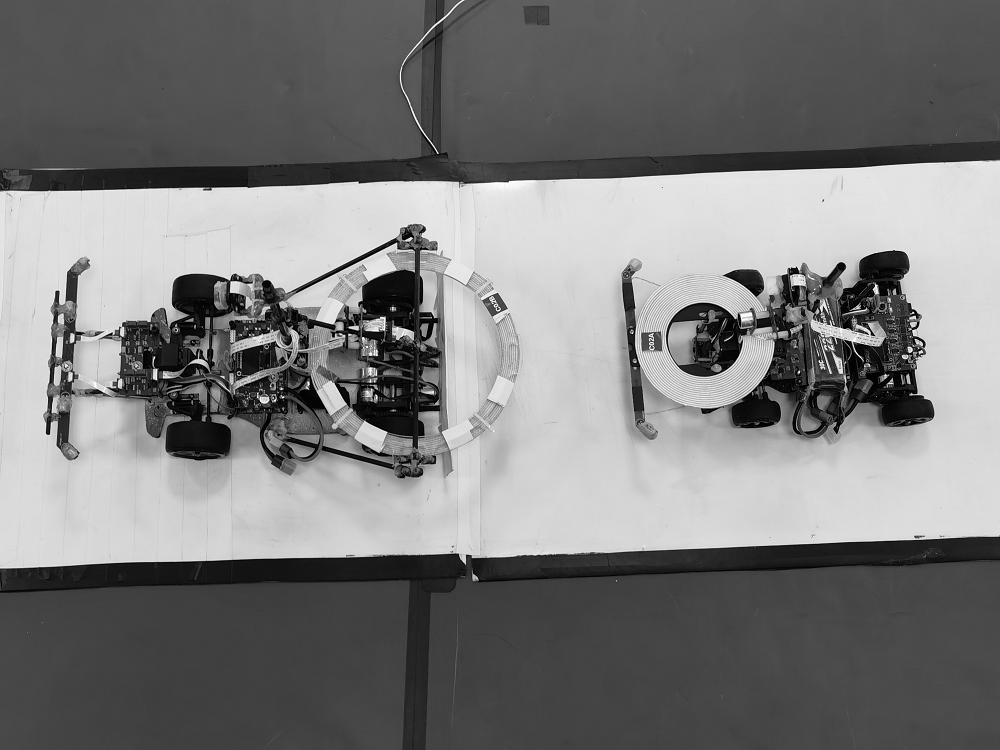
\includegraphics[scale=0.35]{image/actual_compete.png}}
			\caption{双车实际运行图}		
		\end{center}

		\section{结语}
		对智能汽车系统的自主控制,可以分为四大部分:首先是对路径信息的提取与识别,即智能车的寻迹;然后是计算并规划路径,得出可以安全行驶的路径;其次是对车模车速的控制,即智能车的驱动控制;最后,便是最重要的车辆协同性控制,即通过蓝牙以及超声波数据进行双车之间的协同。本文设计并实现了基于图像识别和电磁感应的双车协作智能控制系统,成功实现在识别道路自动循迹和智能避障的基础上完成双车同步协作。本系统利用阿卡曼原理转向和多种pid控制,实现了双车高速跟车速度,通过大津法、贝塞尔曲线\textsuperscript{\cite{ref11}}等图像识别算法和电磁滤波方案,结合动态参数调整,配合全新的定位协作模式,使双车跟随系统具备强稳定性、高安全性和高速度。
				
		\begin{thebibliography}{15}%参考文献
			
			\bibitem{ref1}吴政,韩冰,刘刚.智能汽车自动驾驶的控制方法分析[J].时代汽车,2023(18):7-9.			
			\bibitem{ref2}常彦文.多智能车协同编队与运动规划方法的研究[D].北京石油化工学院,2023.DOI:10.27849.
			\bibitem{ref3}汪秀红(Xiuhong Whang). 低失调高共模抑制比互补双极仪表放大器的研究与设计[D].重庆大学,2022.DOI:10.27670.
			\bibitem{ref4}李子晨. 基于无差拍重复控制的级联H桥APF研究[D].天津理工大学,2022.DOI:10.27360.
			\bibitem{ref5}李杞荣,张文涛,杜浩等.基于FPGA自适应调光的指静脉成像及传输系统[J].工业控制计算机,2023,36(08):61-63+66.
			\bibitem{ref6}李宝芸,范玉刚,高阳.基于OTSU和Canny算子的红外图像特征提取[J].陕西理工大学学报(自然科学版),2019,35(06):33-40.
			\bibitem{ref7}何芝强. PID控制器参数整定方法及其应用研究[D].浙江大学,2005.
			\bibitem{ref8}周润发,杨琦,汪元礼等.基于阿克曼原理的舵机与差速电机协同控制算法的研究与应用[J].赤峰学院学报(自然科学版),2017,33(14):14-15.DOI:10.13398.
			\bibitem{ref9}乔巧. 基于UWB和蓝牙的室内融合定位系统研究与设计[D].华东师范大学,2022.DOI:10.27149.
			\bibitem{ref10}熊永伟.车路协同环境下的车辆自主避撞控制策略研究[D].重庆交通大学,2019.DOI:10.27671.
			\bibitem{ref11}周寅飞,张立华,贾帅东等.最大可航窗口序列约束贝塞尔曲线的无人船自主航行航线规划方法[J/OL].武汉大学学报(信息科学版):1-13[2023-09-27].https://doi.org/10.13203.
		\end{thebibliography}
		
	\end{multicols}%结束分两栏格式
	
		
\end{document}

